\begin{titre}[Représentation et utilisation des solides]

\Titre{Notion de patron, maquette}{1,5}
\end{titre}

 

\begin{CpsCol}
\textbf{Représenter l'espace}
\begin{description}
\item[$\square$] Connaître la notion de patron
\item[$\square$] Construire une maquette
\end{description}
\end{CpsCol}

\Dec{0}{RepS-0}

\begin{DefT}{Prisme Droit}\index{Prisme Droit}

Un \textbf{prisme droit} est un solide de l'espace qui a:
\begin{itemize}
\item deux bases qui sont des polygones de mêmes formes et superposables
\item les autres faces qui sont des rectangles
\end{itemize}
\end{DefT}

\begin{Rq}

Il est caractérisé par ses bases (polygones) parallèles et par sa hauteur.
\end{Rq}

\begin{Ex}
   
\begin{itemize}
\item Le \textbf{cube} est un prisme droit à base carrée et dont la hauteur est égale à la longueur de l'arête du carré de base.

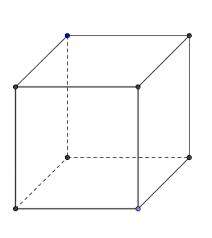
\includegraphics[scale=0.3]{RepS-cube.jpg} 

\item Un \textbf{pavé droit} est un prisme droit à base rectangulaire. L'autre du nom du pavé droit est le \textbf{parallélépipède rectangle}.

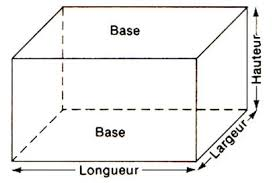
\includegraphics[scale=0.3]{RepS-pave.jpg} 

\item Il existe des prismes droits à base pentagonale, hexagonale, \ldots{}

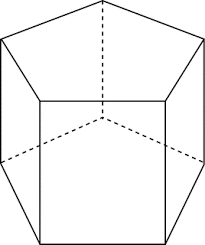
\includegraphics[scale=0.3]{RepS-pentagonale.png} 
\hspace*{1cm}
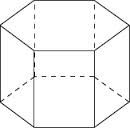
\includegraphics[scale=0.6]{RepS-prisme_hexagonale.jpg}
\hspace*{0.5cm} 
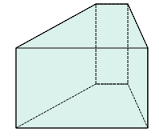
\includegraphics[scale=0.6]{RepS-pirsme_quelconque.png} 
\end{itemize}
\end{Ex}

\begin{Rq}
   
Un cylindre n'est pas un prisme droit car ses faces ne sont pas des polygones.
\end{Rq}

\begin{DefT}{Cylindre}\index{Cylindre}
  
\begin{minipage}{0.48\linewidth}
Un \textbf{cylindre de révolution} est le solide de l'espace obtenu en faisant tourner un rectangle autour d'un axe, appelé \og axe de révolution \fg{}. Il a:
\begin{itemize}
\item deux bases qui sont des disques de mêmes rayons et superposables.
\item l'enveloppe latérale \og dépliée \fg{} est un rectangle. 
\end{itemize}
\end{minipage} 
\hfill
\begin{minipage}{0.48\linewidth}
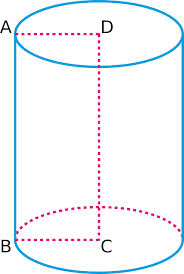
\includegraphics[scale=0.5]{RepS-cylindre.jpg} 
\end{minipage} 
\end{DefT}

\begin{Ex}
   
\begin{itemize}
\item Un cylindre est caractérisé par ses bases (disques) et par sa hauteur
\item Un cylindre n'est pas un prisme droit car ses faces ne sont pas des polygones.
\end{itemize}
\end{Ex}

\begin{DefT}{Pyramides}\index{Pyramides}
    
\begin{minipage}{0.48\linewidth}
Une \textbf{pyramide} est un solide de l'espace qui a:
\begin{itemize}
\item Une base qui est un polygone.
\item Un autre sommet qui n'appartient pas à la base, appelé \og sommet principal \fg{}.
\item Les autres faces qui sont des triangles et qui ont tous en commun le \og sommet principal \fg{}.  
\end{itemize}
\end{minipage} 
\hfill
\begin{minipage}{0.48\linewidth}
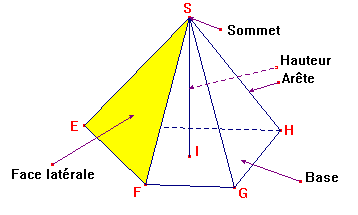
\includegraphics[scale=0.5]{RepS-pyramides_def.png}  
\end{minipage} 
\end{DefT}

\begin{Ex}
    
 
\begin{description}[leftmargin=*]
\begin{minipage}[t]{0.48\linewidth}
\item Une pyramide est caractérisée par sa base et par sa hauteur.
\item Les pyramides en Egypte sont des pyramides à base rectangulaire

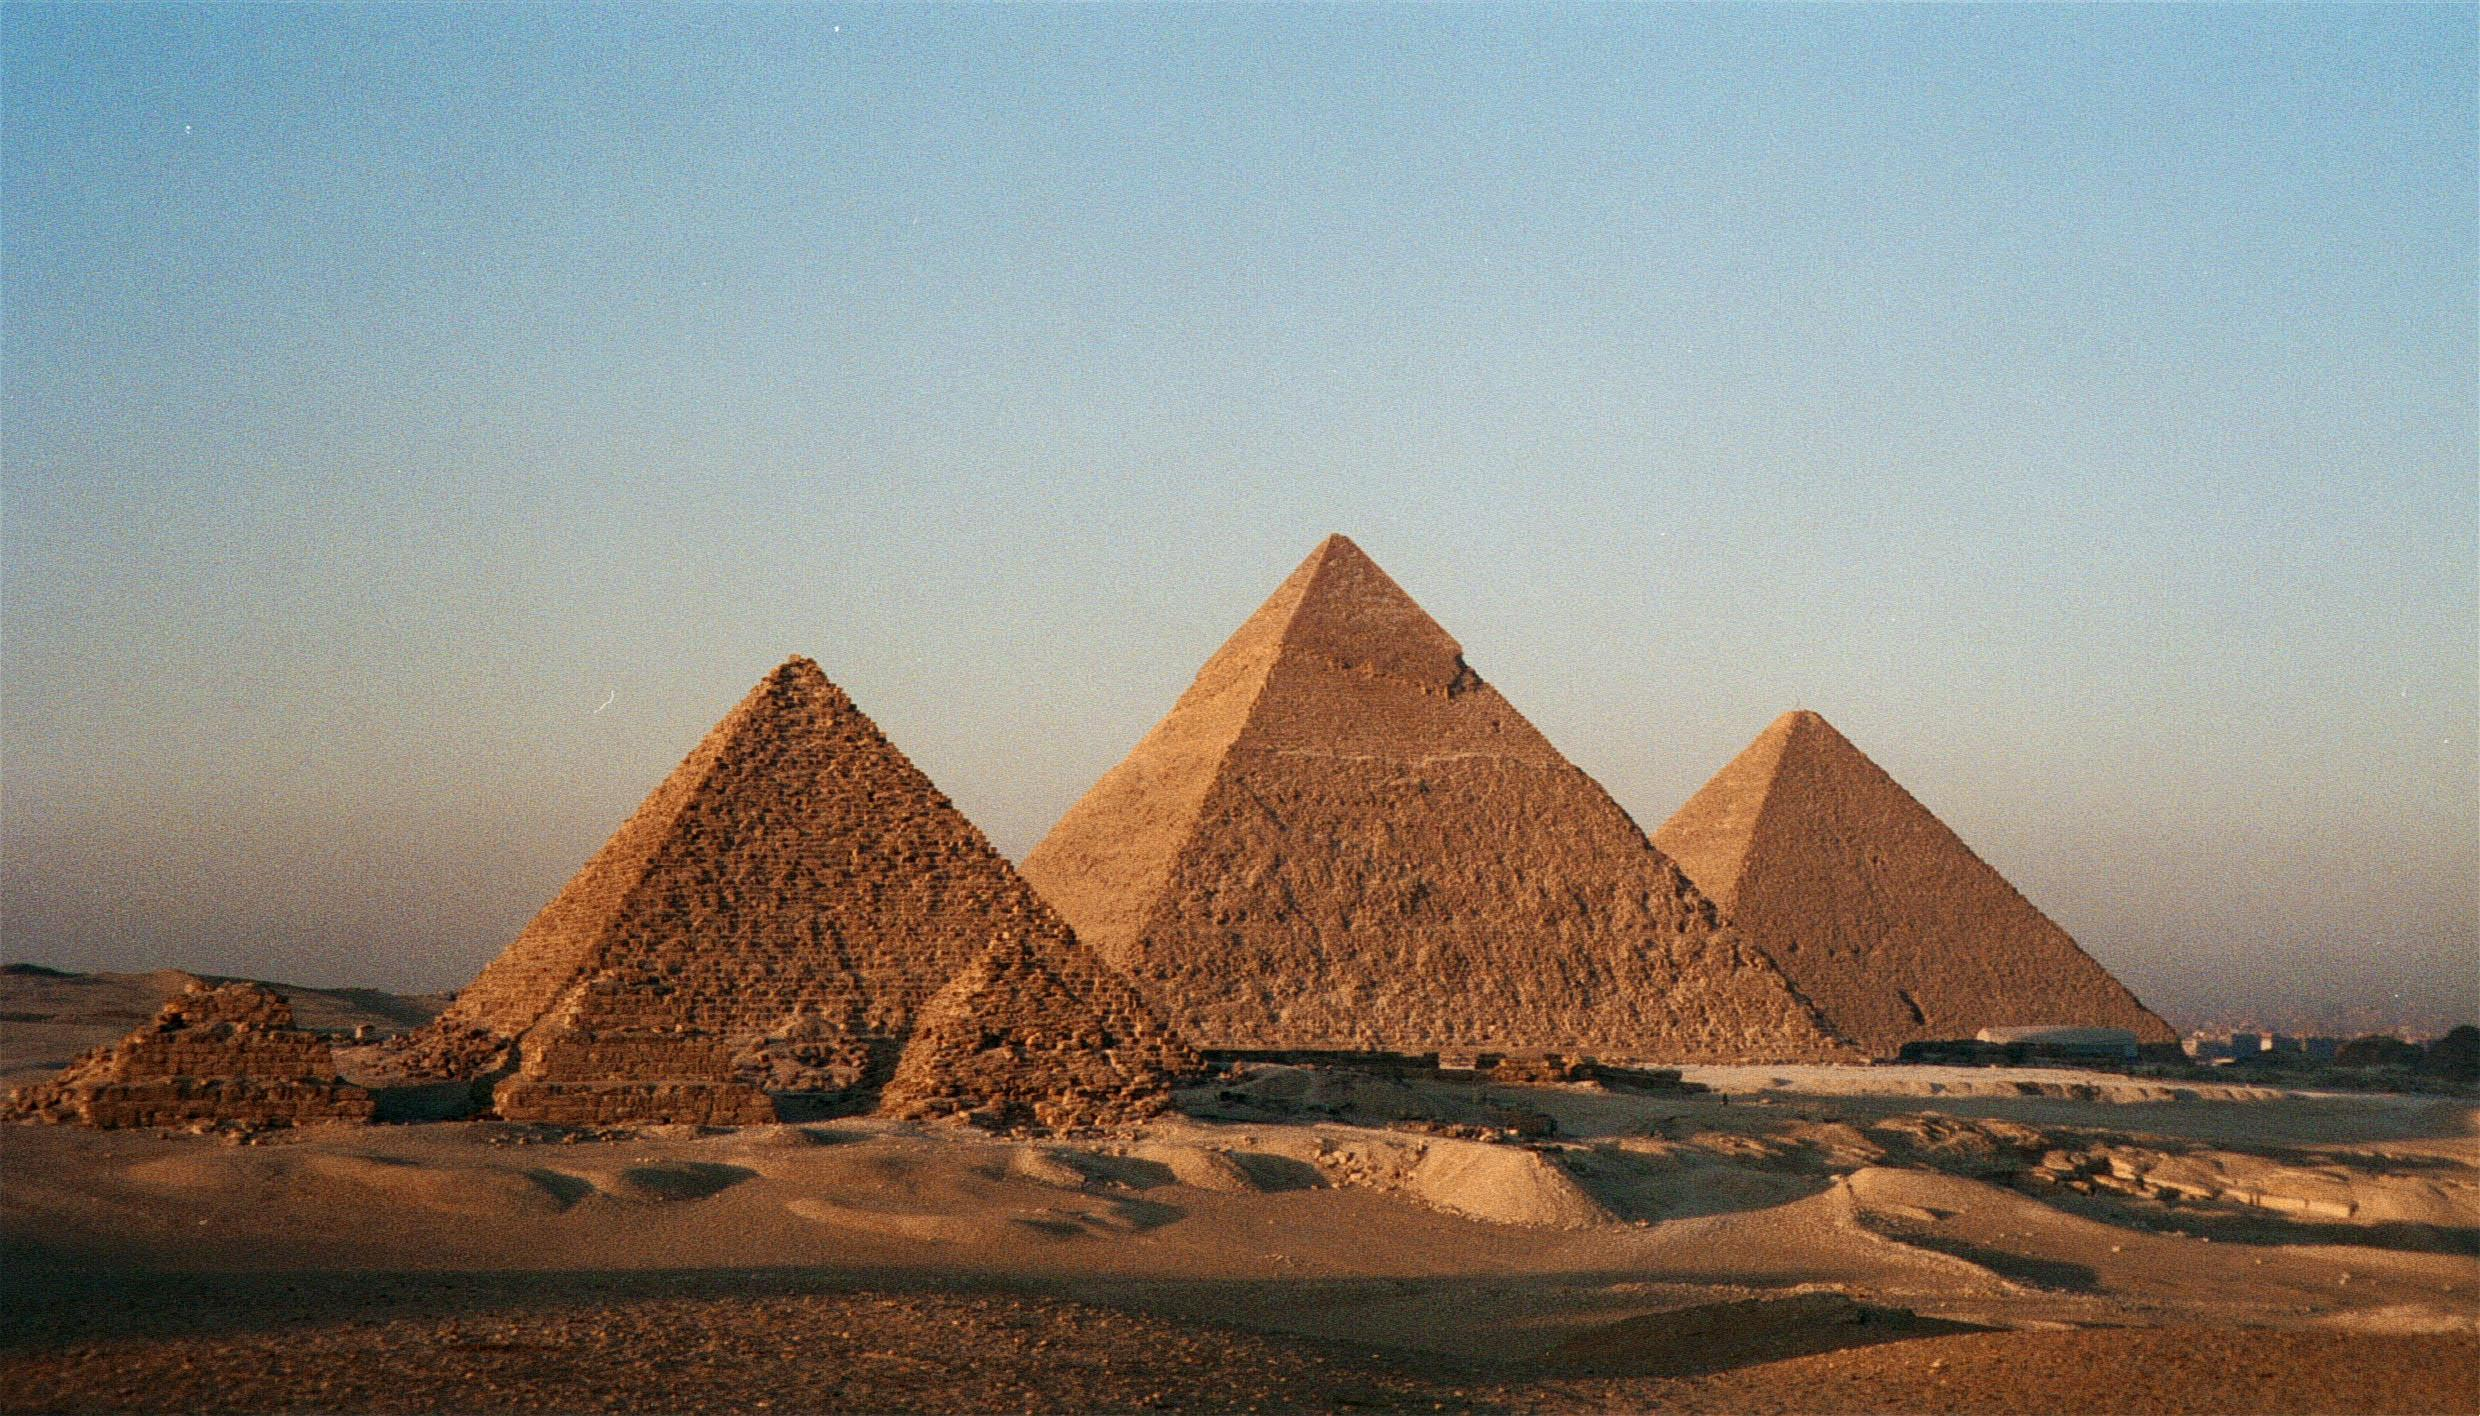
\includegraphics[scale=0.05]{RepS-les-pyramides-d-egypte.jpg} 
\end{minipage} 
\hfill
\begin{minipage}[t]{0.48\linewidth}
\item Voici une pyramide à base octagonale:

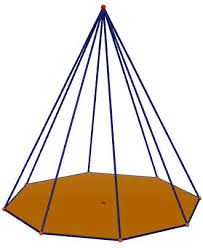
\includegraphics[scale=0.3]{RepS-pyramide_octogonale.jpg} 
\end{minipage}
\end{description}

\end{Ex}

\AD{1}{RepS-22}

\AD{0}{RepS-20}



\Exo{1}{RepS-21}

\begin{DefT}{Cône de révolution}\index{Cône de révolution}
        
Un \textbf{\og cône de révolution \fg{}} est le solide de l'espace obtenu en faisant tourner un triangle rectangle autour d'un axe, appelé \og axes de révolution \fg{}.Il a:
\begin{itemize}
\item Une base qui est un disque.
\item Une enveloppe latérale qui \og dépliée \fg{}  est un secteur angulaire (voir \og construction du patron d'un cône \fg{}) 
\end{itemize}

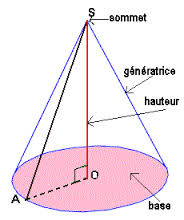
\includegraphics[scale=0.5]{RepS-cone.jpg} 
\end{DefT}

\begin{Rq}
          
Un cône est caractérisé par sa base (disque) et par sa hauteur. 
\end{Rq}

\Exo{1}{RepS-18}

\newpage 

\Exo{1}{RepS-19}

\begin{PpT}{Patron d'un prisme droit}\index{Patron!Prisme droit}

Le \textbf{patron d'un prisme droit} a:
\begin{itemize}
\item deux bases qui sont des polygones identiques.
\item des faces latérales qui sont des rectangles.
\end{itemize}

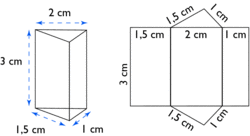
\includegraphics[scale=1]{RepS-patron-prismedroit}


\end{PpT}

\begin{Rq}

\begin{enumerate}
\item Le nombre de rectangle est égal au nombre de faces de la base
\item On commence en général la construction du patron par placer côte-à-côte les rectangles, mais cette construction n'est pas unique
\end{enumerate}

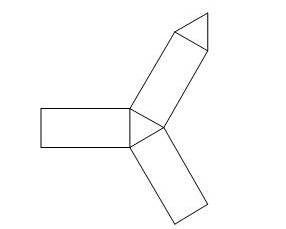
\includegraphics[scale=0.5]{RepS-patron_prismes_eclate.jpg}
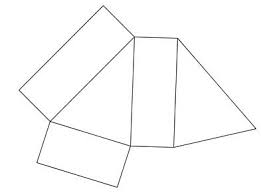
\includegraphics[scale=0.6]{RepS-patron-prismeeclate2.jpg} 

\end{Rq}


\begin{PpT}{Patron d'une Pyramide}\index{Patron!Pyramide}

Le \textbf{patron d'une pyramide} a:
\begin{itemize}
\item Une base qui est un polygone.
\item Des faces latérales qui sont des triangles.  
\end{itemize}
\end{PpT}

\begin{Ex}

Voici le patron d'une pyramide à base rectangulaire:\\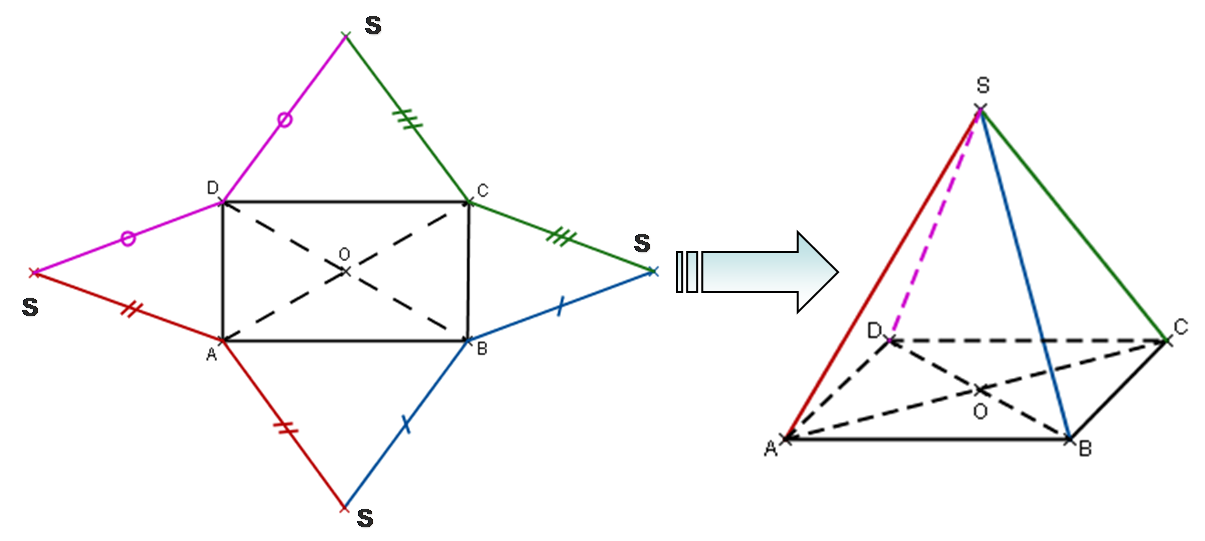
\includegraphics[scale=0.4]{RepS-patron_pyra.png} 

\end{Ex}

\Exo{1}{RepS-24}


\Exo{1}{RepS-23}


\begin{PpT}{Patron d'un Cône de révolution}\index{Patron!Cône de révolution}

\begin{minipage}{0.48\linewidth}
Le \textbf{patron d'un cône} a:
\begin{itemize}
\item Une base qui est un disque.
\item une face latérale qui est un secteur angulaire.  
\end{itemize}
\end{minipage}
 \hfill
\begin{minipage}{0.48\linewidth}
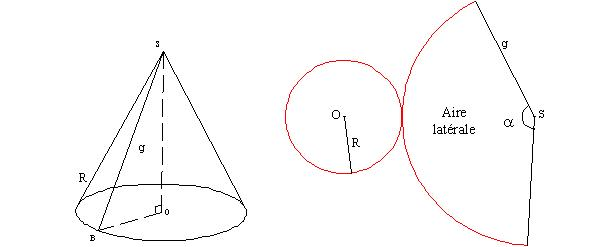
\includegraphics[scale=0.4]{RepS-cone_develope.jpg} 
\end{minipage}
\end{PpT}

\begin{Rq}

Pour calculer l'angle $a$, on utilise un tableau de proportionnalité:
\\%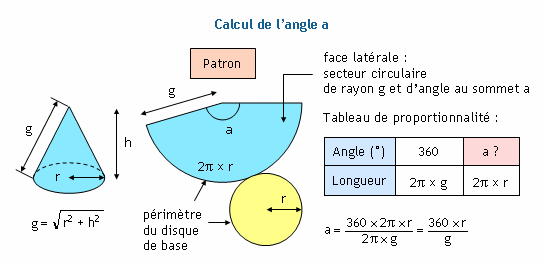
\includegraphics[scale=0.8]{RepS-angle_cone.png} 
\\ $g$ est appelée \og génératrice \fg{} du cône.
\end{Rq}

%

\subsection{Volumes et aires latérales}
\subsubsection{Volumes}
\begin{shaded}
\begin{Pp} 
Le \textbf{volume d'un prisme droit ou d'un cylindre} est calculé par la formule \textbf{$V=B \times h$}, où $B$ est l'aire de la base et $h$ la hauteur
\end{Pp}
\end{shaded}

\begin{Ex}
\begin{itemize}
\item Le volume d'un pavé droit dont la base est un rectangle de dimension $7 cm$ et $6 cm$ et de hauteur $h=5 cm$ est $V=B \times h$ avec $B=7 cm \times 6 cm=42 cm^2$ et $h=5 cm$, donc $V=210 cm^3$
\item Le volume d'un cylindre dont la base est un disque de rayon $7 cm$ et de hauteur $h=5 cm$ est $V=B \times h$ avec $B=\pi \times 7^2 cm^2=49 \pi cm^2$ et $h=5 cm$, donc $V=245 \pi cm^3$. On peut ensuite donner une valeur approchée avec la calculatrice.
\end{itemize}
\end{Ex}

\begin{Rq}
Attention à ne pas confondre pour le cylindre la valeur exacte qui est nécessairement donnée en fonction de $\pi$ et une valeur approchée plus ou moins précise.
\end{Rq}

\begin{shaded}
\begin{Pp} 
Le \textbf{volume d'une pyramide ou d'un cône de révolution} est calculé par la formule \textbf{$V=\frac {B \times h}{3}$}, où $B$ est l'aire de la base et $h$ la hauteur
\end{Pp}
\end{shaded}

\begin{Ex}
\begin{itemize}
\item Le volume d'une pyramide dont la base est un rectangle de dimension $6 cm$ et $5 cm$ et de hauteur $h=4 cm$ est $V=\frac {B \times h}{3}$ avec $B=6 cm \times 5 cm=30 cm^2$ et $h=4 cm$, donc $V=40 cm^3$
\item Le volume d'un cône de révolution dont la base est un disque de rayon $9 cm$ et de hauteur $h=2 cm$ est $V=\frac {B \times h}{3}$ avec $B=\pi \times 9^2 cm^2=81 \pi cm^2$ et $h=2 cm$, donc $V=54 \pi cm^3$. On peut ensuite donner une valeur approchée avec la calculatrice.
\end{itemize}
\end{Ex}

\begin{Rq}
Attention à ne pas confondre pour le cône la valeur exacte qui est nécessairement donnée en fonction de $\pi$ et une valeur approchée plus ou moins précise.
\end{Rq}

\subsubsection{Aires latérales}

\begin{Df} 
\begin{enumerate}
\item \textbf{L'aire latérale d'un prisme ou d'un cylindre} est égale à $A=P \times h$, où $P$ est le périmètre des bases et $h$ la hauteur.
\item \textbf{L'aire latérale d'une pyramide} est égale à la somme des aires des triangles formant les faces latérales.
\item \textbf{L'aire latérale d'un cône} est égale à l'aire d'un secteur angulaire, soit $A=\pi \times r \times g$, où $r$ est le rayon du disque de base et $g$ la longueur de la génératrice.
\end{enumerate}
\end{Df}

\includegraphics[scale=0.7]{aire_laterale_cone.eps} 



\newpage



\section{Exercices}
\begin{Exo}
On considère une pyramide régulière $SABCD$ à
base carrée. On note $[SH]$ sa hauteur et on donne $AH=12$~cm et
$AS=20$~cm.
\begin{enumerate}
\item Calcule la longueur $SH$.
\item Calcule l'angle $\widehat{SAH}$.
\item Montre que la longueur $AB$ est égale à $\sqrt{288}$~cm.
\item Calcule le volume de la pyramide $SABCD$.
\item Construis le patron de la pyramide $SABCD$ à l'échelle
$\dfrac14$.
\item Soit $O$ le point du segment $[SH]$ tel que $SO=6$~cm. On crée
ainsi une deuxième pyramide régulière à base carrée.
\par Calcule le volume de la partie comprise entre les deux pyramides
$SABCD$ et $OABCD$.
\end{enumerate}
\end{Exo}

\begin{Exo}
On considère une pyramide régulière à base carrée $ABCD$ et de sommet
$S$. On note $O$ le centre de la base.
\begin{enumerate}
\item Fais un dessin en perspective cavalière (il n'est pas demandé
  que le dessin soit à l'échelle).
\item On pose $AB=4$~cm et $AS=5$~cm.
\begin{enumerate}
\item En considérant le triangle $ABC$, calcule $AC$. Déduis-en $AO$.
\item Calcule $SO$.
\item Calcule une valeur approchée au mm$^3$ du volume de cette
  pyramide.
\end{enumerate}
\end{enumerate}
%@Commentaire: Exercice qui fait intervenir toutes les notions (sauf le patron) sur les pyramides. Utilisation du théorème de Pythagore dans l'espace.
\end{Exo}

\begin{Exo}
Un cône de révolution de sommet $S$ a un volume de 90~cm$^3$ et une hauteur de 5~cm. Soit $O$ le pied de la hauteur.
\begin{enumerate}
\item Fais un dessin en perspective cavalière.
\item Calcule une valeur approchée au dixième de l'aire de la base.
\item Déduis-en une valeur approchée au millimètre du rayon.
\item Quel serait le volume d'un cône de même rayon et de hauteur 2,5~cm ?
\end{enumerate}
%@Commentaire: Exercice résumant les notions à connaître sur le cône. Résolution d'une équation (question 2).
\end{Exo}

\begin{Exo}
Dans cet exercice, on considère un cône de révolution. Recopie le tableau ci-dessous et effectue les calculs nécessaires pour le compléter. L'unité de longueur est le centimètre. On effectuera les calculs avec $\pi\approx3,14$.
\begin{center}
  \begin{tabular}{|c|c|c|c|c|}
\cline{2-5}
\multicolumn{1}{c|}{}&Rayon de la base&Hauteur&Aire de la base&Volume\\
\hline
Cas 1&3~cm&4~cm&&\\
\hline
Cas 2&&7,2~cm&78,5~cm$^2$&\\
\hline
Cas 3&&&113,04~cm$^2$&376,8~cm$^3$\\
\hline
Cas 4&2~cm&&&11,304~cm$^3$\\
\hline
  \end{tabular}
\end{center}
%@Commentaire: Travail sur la formule de calcul du volume d'un cône. Il y a également un travail sur les équations.
\end{Exo}

\begin{Exo}
Deux récipients ont le même volume.
\begin{itemize}
\item L'un a la forme d'un cylindre de hauteur 10~cm et de rayon de base 6~cm.
\item L'autre a la forme d'un cône de rayon de base 6~cm.
\end{itemize}
\begin{enumerate}
\item Quel est le volume du récipient cylindrique ?
\item Quel est la hauteur du récipient cônique ?
\end{enumerate}
\end{Exo} 





%%%%%%%%%%%%%%%%%%%%%%%%%%%%%%%%%%%%%%%%%%%%%%%%%%%%%%%%%%%%%%%%%%%%%%%%%%%%%%%%%%%%%EXERCICES%%%%%%%%%%%%%%%%%%%%%%%%%%%%%%%%%%%%%%%%%%%%%%%%%%%%%%%%%%%%%%%%%%%%%%%%%%%%%%%%%%%%%%%%%%%%%%%%%%%%%%%%%%%%%%%%%%%%%%%%%%%%%%%%%%%%%%%%%%%%



%\AD{1}{RepS-28}


\mini{
\Exo{1}{RepS-25}
}{
\Exo{1}{RepS-26}
}
\Exo{0}{RepS-45}

\Rec{1}{RepS-27}

%\begin{autoeval}
%\begin{tabular}{p{12cm}p{0.5cm}p{0.5cm}p{0.5cm}p{1cm}}
%\textbf{Compétences visées} &  M I & MF & MS  & TBM \vcomp \\ 
%Connaître la notion de patron & $\square$ & $\square$  & $\square$ & $\square$ \vcomp \\
%Construire une maquette & $\square$ & $\square$  & $\square$ & $\square$ \vcomp \\  
%\end{tabular}
%{\footnotesize MI : maitrise insuffisante ; MF = Maitrise fragile ; MS = Maitrise satisfaisante ; TBM = Très bonne maitrise}
%\end{autoeval}